% -*- mode: latex; fill-column: 80; -*-
\documentclass[a4paper,10pt]{report}

\hoffset=-0.75in
\voffset=-1in
\textwidth=450pt
\textheight=720pt

\usepackage{hyperref}
\hypersetup{
  colorlinks,
  citecolor=blue,
  filecolor=blue,
  linkcolor=blue,
  urlcolor=blue
}

\usepackage{graphicx}
\graphicspath{ {./image/} }

\usepackage{subcaption}

\def\FlintVersion{2.0}
\def\Flint{Flint \FlintVersion}
\def\Tagline{a simulator for biological and physiological models}

\newcommand\FigureOfImage[2]{\begin{figure}[h]
  \centering
  \includegraphics[width=0.8\textwidth]{#1}
  \caption{#2}\label{fig:#1}
\end{figure}}

\title{\Flint: The User Guide}
\author{Flint project}

\makeindex

\begin{document}

\maketitle

\begin{abstract}
This document describes how to use \Flint.
Readers also find some OS-specific notes and trouble-shooting techniques which
users would like to know when using \Flint.
\end{abstract}

\tableofcontents


%%%%%%%%%%%%%%%%%%%%%%%%%%%%%%%%%%%%%%%%%%%%%%%%%%%%%%%%%%%%%%%%%%%%%%%%

\chapter{Introduction}

\section{Brief summary about Flint}
\Flint~is new reimplementation of Flint 1.x, \Tagline.
Flint can run simulations of multi-level physiological models written in PHML.
It means that Flint parses given models, performs numerical analysis for their
simulation, and renders simulation outcome into a line graph via an external
program such as gnuplot \cite{gnuplot}.
Likewise, Flint can handle CellML and SBML as well as SBML-PHML hybrid models.

\subsection{Markup languages}
\Flint\ supports the following standard languages for models:
\begin{itemize}
\item PHML \cite{PHML} (including its precursor ISML \cite{ISML})
\item SBML \cite{SBML}
\item CellML \cite{CellML} (as an experimental feature)
\end{itemize}

\subsection{Solver methods for ordinary differential equations}
\Flint\ supports the following two algorithms to solve ODEs numerically:
\begin{itemize}
\item Euler method
\item Runge-Kutta 4th-order method
\item Adaptive stepsize Runge-Kutta method, based on the ARKode solver of
  SUNDIALS \cite{hindmarsh2005sundials}
\end{itemize}

\section{Notation}
In this document, a sentence starting with {\tt \$} describes a command line in
a command shell on your system, such as\\
{\tt \$ echo this is a command line.}


%%%%%%%%%%%%%%%%%%%%%%%%%%%%%%%%%%%%%%%%%%%%%%%%%%%%%%%%%%%%%%%%%%%%%%%%

\chapter{Getting started}

\section{Install \Flint}
Flint project makes both Windows and macOS version of \Flint\ freely
available at \url{https://flintproject.github.io/}.
The .dmg archive for macOS contains Flint's application bundle, named
``Flint.app''; extracting it and copying it into your favorite path is all
you have to do for installation.
For Windows, double-clicking the .msi package will start the installation
process.

\section{Try your first simulation with \Flint}
This section describes a simple procedure with \Flint\ to run a simulation of an
example model ``HodgkinHuxley\_1952\_neuron\_model.phz'', which is distributed
as part of the PhysioDesigner \cite{PhysioDesigner} installation.

\begin{description}
\item[Launch Flint] \hfill \\
To launch Flint, double-click flint.exe on Windows, or Flint.app on macOS.
It shows a window like Fig.~\ref{fig:initial}.
\FigureOfImage{initial}{The initial window of Flint.}

\item[Open a model] \hfill \\
In the ``File'' menu, select ``Open'' to choose a model file. Then you will see
a file dialog like Fig.~\ref{fig:open-model}.
\FigureOfImage{open-model}{The file dialog to open a model.}
Select ``HodgkinHuxley\_1952\_neuron\_model.phz'' in the file dialog, and
click ``Open'' button.
Then the model window will appear as in Fig.~\ref{fig:hh}.
\FigureOfImage{hh}{The model window.}

\item[Choose duration and time step] \hfill \\
Specify the duration of simulation in ``Simulation Length'' and the time step
length of the simulation in ``Simulation Time Step'' optionally.

\item[Run a simulation] \hfill \\
Click the ``Run'' button to start a simulation.

Once simulation started running, the progress bar will appear in the control
panel in the right side like Fig.~\ref{fig:hh-progress}, and both the cross mark
(as ``Cancel'') and ``Detail'' buttons will be enabled.
\FigureOfImage{hh-progress}{The progress bar for the model.}

Wait until the status bar tells that the simulation completed (see
Fig.~\ref{fig:hh-compeleted}).
\FigureOfImage{hh-completed}{The status bar indicates the simulation completed.}

\item[See detail of the simulation] \hfill \\
Click the ``Detail'' button to get the simultion result.
Then a detail window will appear as in Fig.~\ref{fig:hh-detail}.
\FigureOfImage{hh-detail}{The detail window.}

\item[Select ordinates] \hfill \\
Click the ``View'' button on the detail window, then a plot window to render
line graphs about the simulation result, like Fig.~\ref{fig:hh-plot}.
\FigureOfImage{hh-plot}{The plot window.}
Check the Y1 column of ``V'' in the variable list, which calls gnuplot.
Soon the corresponding line graph will appear on a separate window,
like Fig.~\ref{fig:hh-plot-v}.
\FigureOfImage{hh-plot-v}{The plot window with ``V'' on Y1.}
Moreover you can also check the Y2 column of another variable ``I\_Na'' in the
list to arrange two line graphs in the same canvas, as in
Fig.~\ref{fig:hh-plot-v-ina}.
\FigureOfImage{hh-plot-v-ina}{The plot window with ``V'' on Y1 and ``I\_Na''
on Y2.}
\end{description}


%%%%%%%%%%%%%%%%%%%%%%%%%%%%%%%%%%%%%%%%%%%%%%%%%%%%%%%%%%%%%%%%%%%%%%%%

\chapter{Graphical User Interface}
\Flint\ comes with a graphical user interface out of the box. This chapter
explains features of the GUI and how to use them.

\section{Launching Flint}
On Windows, double-clicking ``flint.exe'' in the start menu starts Flint.
On macOS, double-clicking ``Flint.app'' works similarly.

\section{Quitting Flint}
To quit Flint, use the menu ``File''$\rightarrow$``Exit''.

\section{Loading models}
Flint must load models before running simulations for them.
Users tell Flint which model should be loaded by opening the model file.
Loading a model can fail due to some reasons; for example, it may fail if
the model file contains an error or unsupported elements.
An error dialog will display a diagnosis message when loading a model fails.
Once loading a model successfully, the model window shows up and stays
in the main window until closed, like Fig.~\ref{fig:lr}.

\section{Configuring simulation tasks}
\FigureOfImage{lr}{The model window.}
Before starting simulations for a loaded model, users may want to configure them
in terms of numerical integration, simulation time, output data, and parameters.

\subsection{Integration method}
Users have to choose a solver method for ordinary differential equations at the
``Integration method'' combobox.

\subsection{Simulation Length}
Users must specify the total length of simulation time at the ``Simulation Length''
field; the given number is interpreted in terms of the selected time unit.

\subsection{Simulation Time Step}
Similarly to ``Simulation Length'', users can specify the time step at the
``Simulation Time Step'' field.

\subsection{Starting from}
Users can specify when (in the sense of simulation time) output starts from
at this field. By default, simulation process produces output from time 0.

\subsection{Data Sampling}
This setting is for determining how often the result data are written in.
Note that the sampling rate does not affect the calculation for simulation.

\subsection{Select output variables}
Before starting simulations for a loaded model, users may want to choose a
limited number of variables for output among available variables.
Filtering output variables will reduce the burden of writing output, and thus
may improve the simulation performance.
The ``Output Variables'' panel (Fig.~\ref{fig:lr-output-variables}) allows
user to select output variables by matching its properties, such as name,
with a given string.
\FigureOfImage{lr-output-variables}{The ``Output Variables'' panel.}

\subsection{Parametrize constant values}
By default, Flint run a simulation job for a loaded model. At the same time
it is possible to run a bunch of simulations at once for a single model with
different values of parameters.

A parameter is bound to a set of possible values, called value-set.
The whole set of possible tuples of multiple parameters is defined as a
cartesian product of multiple value-sets.
If users edit parameter sets and use them, then Flint will run as many jobs
for the model as cardinality of the cartesian product. In other words,
each simulation job corresponds to a value tuple for multiple parameters.

Users can see and modify parametrization of constant elements in a loaded model,
such as the initial values of ordinary differential equations and values of
static-parameters of PHML, at the ``Parameters'' panel.

The table at the ``Parameters'' consists of each row corresponding to a constant
element in the model; the ``Expression'' field of the row accepts a formula
(in an infix notation) defining the parametrized value of the constant element.

\begin{figure}[h]
  \centering
  \begin{subfigure}[b]{0.45\textwidth}
    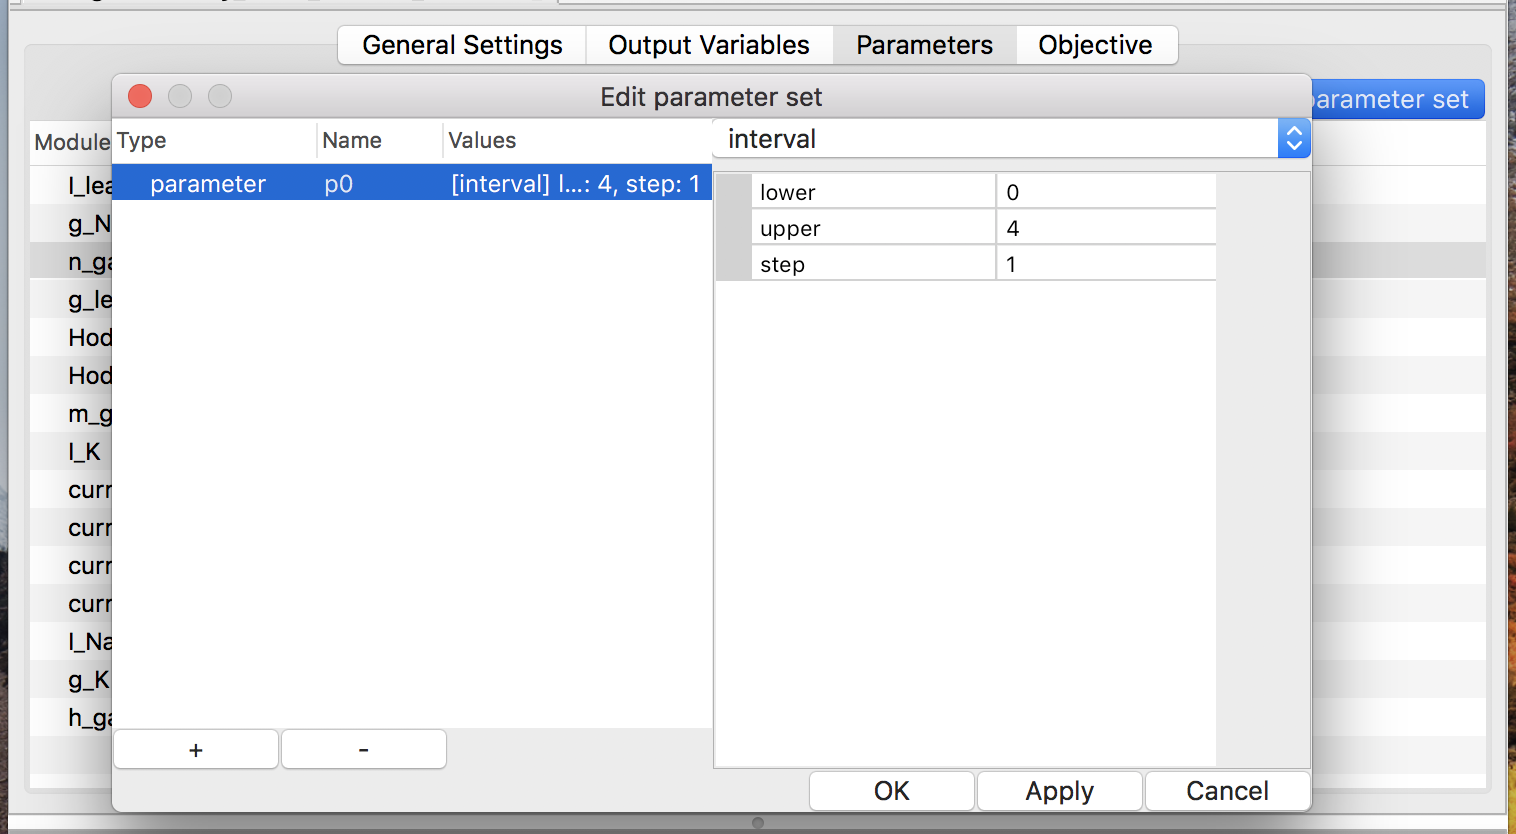
\includegraphics[width=\textwidth]{lr-edit-parameter-set-a}
    \caption{{\tt a} edit a parameter set calld ``p0''}\label{fig:lr-edit-parameter-set-a}
  \end{subfigure}
  \begin{subfigure}[b]{0.45\textwidth}
    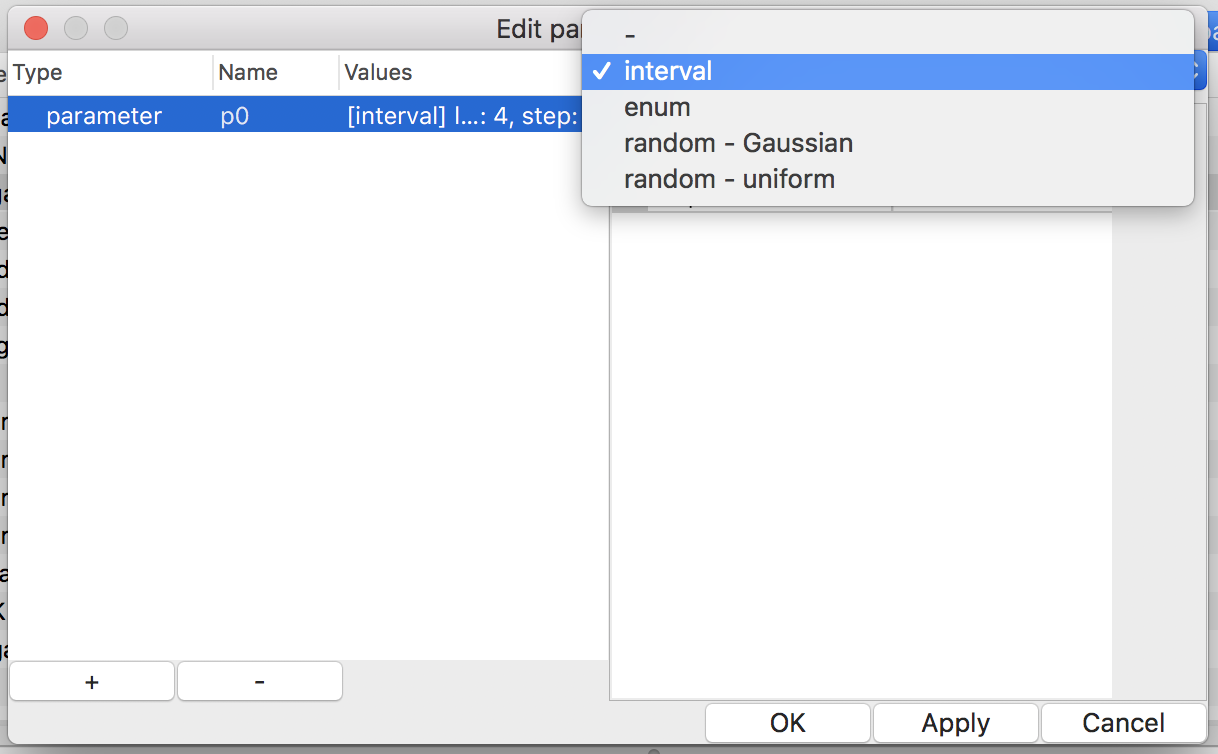
\includegraphics[width=\textwidth]{lr-edit-parameter-set-b}
    \caption{{\tt b} choosing value type}\label{fig:lr-edit-parameter-set-b}
  \end{subfigure}
  \caption{Editing parameter sets in the ``Define parameter set'' window.}
\end{figure}

\subsubsection{Define a value-set}
In order to define or modify value-sets, push button ``Define value set'' at
first. Then a window will pop up. It allows users to define new value-set,
see existing value-sets, and modify them (see Fig.~\ref{fig:lr-edit-parameter-set-a}).

There are four types of value-sets: enum, interval, Gaussian, and uniform
(see Fig.~\ref{fig:lr-edit-parameter-set-b}).
For a value-set of type enum, each of possible values must be specified.
On the other hand, only the lower and upper (both inclusive) of a range
of values with a step are required to define a value-set of type interval.
Note that possible values of an enum should be separated by a comma.
The latter two types of value-sets are for generating (pseudo)random values
according to specified probability distribution in simulation time.

\subsubsection{Use value-sets}
Once users have defined a value-set, it is available in the ``Expression''
field of any row in the ``Parameters'' table. For example, users can specify
{\tt a+2*b} in the field if there exists a couple of value-set named {\tt a} and
{\tt b} (see Fig.~\ref{fig:lr-parameter-set}).
\FigureOfImage{lr-parameter-set}{Parameterize with defined value-set ``p0''.}

\section{Starting simulation}
To start simulation, use the menu ``Control''$\rightarrow$``Run'' or button
``Run'' on the control panel. It kicks simulation jobs for all loaded models.
Users can monitor the progress in total on the control panel, as well as the
one for a single job on the detail windows like Fig.~\ref{fig:lr-detail}.
Note that a context menu allows users to cancel simulation assigned to a
specific parameter value in a task.
\FigureOfImage{lr-detail}{The detail window during simulation.}

\section{Controlling simulation jobs}
After starting simulation jobs, users can control them instead of just waiting
for them finishing.

\subsection{Cancel jobs}
There is another way to cancel running jobs; pushing the cross mark on the
control panel (see Fig.~\ref{fig:lr-progress}), which cancels a job i.e. all
of its tasks together.
\FigureOfImage{lr-progress}{The progress bar / cross mark / ``Detail'' button on
 the control panel.}

\subsection{Pause and resume jobs}
As in Fig.~\ref{fig:control}, users can pause jobs at any time during simulation
by using the menu ``Control''$\rightarrow$``Pause''. Resumeing paused jobs can
be done with the menu ``Control''$\rightarrow$``Resume''.
Note that these operation affects all of alive jobs simultaneously.
\FigureOfImage{control}{The Control Menu.}

\section{Visualizing simulation results}
Flint has a feature to show a line graph for the result of a simulation on the
fly, not only after its job finished, but also int the middle of ongoing
simulation.

From the detail window, users can display the plot window by clicking button
``View'' for each simulation job.

\subsection{Choose abscissa and ordinates}
In order to draw a line graph, users have to specify the abscissa and ordinates
by checking an X column as well as either Y1 or Y2 column.
Immediately after choosing abscissa and ordinates, Flint calls gnuplot in the
background to draw a line graph.
Thus users have to install gnuplot in advance, and to specify the location of
the gnuplot executable (see section~\ref{sec:preference}).

\subsubsection{Trouble shooting}
\begin{itemize}
\item Choosing abscissa and ordinates results in no response, make sure if the
  gnuplot initialization file is valid and correct.
  It is called $\tt{.gnuplot}$ on Unix and macOS, and $\tt{GNUPLOT.INI}$ on
  other systems.
\end{itemize}

\section{Saving output data}
Users may save the resulting simulation data for later investigation.
\FigureOfImage{lr-export}{The dialog to save data.}

\subsection{Exporing data as CSV}
Flint can export the result data into a CSV file.
The header column contains the variable names as well as their unit name if any.

The procedure is as follows:
\begin{enumerate}
\item Open the ``Detail'' window
\item Select as many tasks as you would like to save.
\item Push button ``Export''
\item Choose a target directory in the file dialog (see Fig.~\ref{fig:lr-export})
\end{enumerate}
The names of files saved in the target directory are of form ``(ID).csv.''

\subsection{Exporting data as ISD}
Flint can also export the result data into a ISD file.
The ISD file format is a binary file format for preserving multi-variate data.

The procedure is as follows:
\begin{enumerate}
\item Open the ``Detail'' window
\item Select as many tasks as you would like to save.
\item Push button ``Export''
\item Choose a target directory in the file dialog (see Fig.~\ref{fig:lr-export})
\end{enumerate}
The names of files saved in the target directory are of form ``(ID).isd.''

\section{Exporting C source code from model}
Not only running online simulation, but also Flint can export simulation code
as a C99 source file from a loaded model. So far it works only for pure ODE models.

\subsection{From menu}
To export C code from a model,
\begin{enumerate}
\item Load a model
\item Select the menu ``File''$\rightarrow$``Export to C'' (see Fig.~\ref{fig:export-to-c})
\item Choose a target filename via the file dialog that follows.
\end{enumerate}
\FigureOfImage{export-to-c}{The menu ``File''$\rightarrow$``Export to C''.}
Then a dialog will appear to tell whether it is done successfully or not.

Please note that the numerical method used in the exported code is the one
specified in the original model, e.g., Euler or Runge-Kutta 4th-order method;
the ARKode solver of SUNDIALS has not been supported yet.

\subsection{How to build a program from exported code}
Once a C source file exported, what to do next is building the program by a C compiler
conforming C99 standard.

If, for example, gcc is available, then invoking the following code
\begin{verbatim}
$ gcc -O3 -std=c99 -o simulate exported.c
\end{verbatim}
will produce an executable named {\tt simulate} from the C source file {\tt exported.c}.

Finally,
\begin{verbatim}
$ ./simulate output.isd
\end{verbatim}
will run a simulation, writing the whole output into {\tt output.isd}.

\section{Preference}
\label{sec:preference}
Users can customize Flint's behavior via preference, which UI looks like
Fig.~\ref{fig:preference-plotter}.

\subsection{Plotter}
This is a necessary option to render line graphs.
Select the path of {\tt gnuplot} (or {\tt gnuplot.exe} on Windows), e.g.,
``$\tt{/usr/bin/gnuplot}$''. If macOS users have, say,
{\tt /Applications/gnuplot.app} as an application bundle of gnuplot,
its value should be \[{\tt /Applications/gnuplot.app/bin/gnuplot}.\]
\FigureOfImage{preference-plotter}{The ``Plotter'' panel on the preference dialog.}

\section{Shortcut keys}
There are useful shortcut keys as follows:

\subsection{Keys for main menu}
\begin{tabular}{l||c|c}
  Command & Shortcut keys on macOS & Shortcut keys on Linux or Windows\\
  \hline
  File $\rightarrow$ Open & {\tt Cmd}+O & {\tt Ctrl}+O \\
  File $\rightarrow$ Exit & {\tt Cmd}+Q & {\tt Ctrl}+Q \\
  Edit $\rightarrow$ Copy & {\tt Cmd}+C & {\tt Ctrl}+C \\
  File $\rightarrow$ Cut  & {\tt Cmd}+X & {\tt Ctrl}+X \\
  Edit $\rightarrow$ Preference & {\tt Cmd}+, & {\tt Ctrl}+, \\
  Control $\rightarrow$ Run & {\tt Option}+R & {\tt Alt}+R \\
  Control $\rightarrow$ Pause & {\tt Option}+P & {\tt Alt}+P \\
  Control $\rightarrow$ Resume & {\tt Option}+S & {\tt Alt}+S \\
\end{tabular}

\subsection{Additional keys}
Both {\tt Esc} and {\tt Ctrl}+{\tt W} (or {\tt Cmd}+{\tt W} on Mac) can close an active
subwindow in which there is no dedicated button to close it.

%%%%%%%%%%%%%%%%%%%%%%%%%%%%%%%%%%%%%%%%%%%%%%%%%%%%%%%%%%%%%%%%%%%%%%%%

\chapter{Command Line Interface}
\Flint\ allows users to run a simulation in a command shell.

\section{Launching Flint}

\subsection{Invocation with no arguments}
It is possible to launch Flint with the command {\tt open(1)} of macOS as follows:
\begin{verbatim}
$ open Flint.app
\end{verbatim}
Note that it does nothing but launches the graphical user interface of Flint.
In a {\tt cmd} session on Windows,
\begin{verbatim}
$ flint.exe
\end{verbatim}
has the similar effect.

\subsection{Invocation with filenames}
If filenames of models are given in the command line on Windows:
\begin{verbatim}
$ flint.exe model1 model2 ...
\end{verbatim}
then Flint tries to open them immediately after launching the GUI.

\section{Showing help}
Specifying {\tt -help} in the command line shows the help message.

\subsection{Synopsis}
On Windows:
\begin{verbatim}
$ flint.exe -help
\end{verbatim}

\section{Running a simulation: the headless mode}
Specifying {\tt -headless} in the command line enable the headless mode, which
runs a simulation of given model with the default configuration.

\subsection{Synopsis}
On Windows:
\begin{verbatim}
$ flint.exe -headless input output [-e file] [-g n] [-s file]
\end{verbatim}
Load a model at {\tt input}, simulation it with the default configuration,
and leave the result at {\tt output}.
The following suboptions are available:
\begin{description}
\item[-e {\tt file}] \hfill \\
  save error messages during simulation as {\tt file}.
\item[-g {\tt n}] \hfill \\
  specify output sampling rate i.e. 1 output per {\tt n} step.
\item[-s {\tt file}] \hfill \\
  specify output variables with {\tt file}.
\end{description}

%%%%%%%%%%%%%%%%%%%%%%%%%%%%%%%%%%%%%%%%%%%%%%%%%%%%%%%%%%%%%%%%%%%%%%%%

\chapter{Frequently Asked Questions (FAQ)}
Please read this chapter first when in doubt.

\section{How to uninstall Flint}
On windows, you can uninstall Flint through the system menu ``Settings''$\rightarrow$``Apps \& features''.
On macOS, all you have to do for uninstallation is to remove Flint.app.

%%%%%%%%%%%%%%%%%%%%%%%%%%%%%%%%%%%%%%%%%%%%%%%%%%%%%%%%%%%%%%%%%%%%%%%%

\bibliographystyle{unsrt}
\bibliography{publication,software}

\end{document}
